\documentclass[letterpaper,12pt]{article}
\usepackage[utf8]{inputenc}
\pagestyle{plain}
\usepackage{graphicx}
\usepackage[small]{caption}
\usepackage{cite}
\usepackage{amsmath}
\usepackage{multirow}
\usepackage{setspace}
\usepackage{xcolor}
\usepackage{authblk}
\usepackage{url}
\usepackage{hyperref}

\pagenumbering{roman}
%Insert your title and author list below
\title{Light Meson Form Factors from \textbf{D}eep \textbf{E}xclusive \textbf{M}eson \textbf{P}roduction in early EIC science configurations with the ePIC Detector}
\author[1]{G.M. Huber}
\author[2]{S.J.D. Kay}
\author[1]{L. Preet}

\affil[1]{Department of Physics, University of Regina, SK, S4S 0A2, Canada}
\affil[2]{School of Physics, Engineering and Technology University of York, YO10 5DD, UK}
\date{MONTH 2025}

\begin{document}

\maketitle
\begin{abstract}
Abstract goes here
\end{abstract}

\begin{figure}[h]
    \centering
    
\includegraphics[scale=0.5]{Figures/EPIC-logo_black.png}
\end{figure}

\pagebreak
\tableofcontents

\pagebreak
\pagenumbering{arabic}

\section{Introduction}\label{sec:Intro}


Pions and kaons are among the most prominent strongly interacting particles next to the nucleon, since they are the Goldstone bosons of QCD. Thus, it is important to study their internal structure and how this reflects their Goldstone boson nature; a question particularly relevant for understanding the origin of mass generation in QCD.  

The hard contribution to the $\pi^+$ form factor can be calculated exactly within the framework of pQCD, and at asymptotically high $Q^2$ it takes a particularly simple form, $F_{\pi}(Q^2) \overrightarrow{_{Q^2 \rightarrow \infty}} 16 \pi \alpha_s(Q^2)f_{\pi}^2/Q^2$ \cite{PETERLEPAGE1979359}, where $f_{\pi}$ is the $\pi^+$ decay constant.  In general, the pion also contains soft contributions, which are expected to dominate at lower $Q^2$. The actual behavior of $F_{\pi}$ as a function of $Q^2$, as QCD transitions smoothly from the non-perturbative (long-distance scale) confinement regime to the perturbative (short-distance scale) regime, is an important test of our understanding of QCD in bound hadron systems. Since QCD calculations cannot yet be performed rigorously in the confinement regime, experimental data from JLab play a vital role in validating the theoretical approaches employed. In particular, due to the charged pion's relatively simple quark-antiquark ($q\bar{q}$) valence structure and its experimental accessibility, the pion elastic form factor ($F_{\pi}$) offers our best hope of directly observing QCD's transition from color-confinement at long distance scales to asymptotic freedom at short distances. It is worth highlighting that in QCD the difference between the kaon and pion charge form factors is of the scale of 20\% at $Q^2 \sim$ 5 GeV$^2$~\cite{Gao:2017mmp} and disappears at asymptotic $Q^2$ as ln($Q^2$).  Thus, the acquisition of experimental data for both form factors covering a wide $Q^2$ range should be a high priority.

Current experimental information on the pion and kaon form factors is limited, particularly at large $Q^2$ \cite{Horn:2016rip}. Measurement of the $\pi^+$ electromagnetic form factor for $Q^2>0.3$ GeV$^2$ can be accomplished by the detection of the exclusive reaction $p(e,e'\pi^+)n$ at low $-t$. This is best described as quasi-elastic ($t$-channel) scattering of the electron from the virtual $\pi^+$ cloud of the proton, where $t=(p_{p}-p_{n})^2$ is the Mandelstam momentum transfer to the target nucleon. Scattering from the $\pi^+$ cloud dominates the longitudinal photon cross section ($d\sigma_L/dt$),  when $|t|\ll m_p^2$. To reduce background contributions, one preferably separates the components of the cross section due to longitudinal (L) and transverse (T) virtual photons (and the LT, TT interference contributions), via a Rosenbluth separation.  

A Rosenbluth separation involves the absolute subtraction of two measurements determined at high- and low-virtual photon polarization ($\epsilon_{Hi}$, $\epsilon_{Lo}$), corresponding to high and low electron beam energies, with very different detector rates. The resulting errors on $\sigma_L$ and $\sigma_T$ are magnified by $1/\delta\epsilon=(\epsilon_{Hi}-\epsilon_{Lo})^{-1}$. To keep the uncertainties in $\sigma_L$ to an acceptable level, $\delta\epsilon >0.2$ is typically required, {\it i.e.} an uncertainty magnification of no more than 5. The measurements require continuous, high intensity electron beams, and detectors with good particle identification and reproducible systematics. JLab Hall~C is currently the only facility worldwide capable of such studies.  

At the EIC, $\pi^+$ form factor measurements can be extended to significantly larger $Q^2$ than possible at JLab.  We have written an exclusive $p(e,e'\pi^+n)$ event generator~\cite{DEMPgen} and performed detailed simulations to determine the feasibility of $F_{\pi}$ measurements at the EIC\@.  The key questions we have addressed include: 1) detector requirements to cleanly identify exclusive $e' \pi^+ n$ coincidences; 2) experimental acceptance and projected counting rates for such triple coincidences; 3) event reconstruction resolution requirements to reliably extract $F_{\pi}(Q^2)$ from $p(e,e'\pi^+n)$ data. Since the cross section falls rapidly as the distance from the pion pole $(t-m_{\pi}^2)$ is increased, this steep fall off needs to be measured to confirm the dominance of the pion cloud mechanism in the acquired data. This note describes our work addressing all of these questions and evaluating what can be achieved with the EIC in its first five years of running.

\section{Simulation Overview}\label{sec:Sim_Overview}

The analysis presented in this note utilises our event generator, DEMPgen \cite{DEMPgen}, in conjunction with the ePIC software stack to produce projections for pion form factor measurements at the EIC. Details on the event generator, simulation and subsequent reconstruction are presented in this section.

\subsection{Event Generator Details}\label{subsec:EvGen}

\href{https://github.com/JeffersonLab/DEMPgen/releases}{DEMPgen version 1.2.4}\footnote{\url{https://github.com/JeffersonLab/DEMPgen/releases}} was utilised to generate $p(e,e'\pi^+n)$ events for this study. DEMPgen events are absolutely-normalized so that project event rates can easily be predicted. This normalization is maintained in the form of an event weighting which is retained through the simulation and reconstruction chain before being applied to final results. Two different early science configurations were studied, namely $10$~GeV electron on $130$~GeV (10x130) proton and $10$~GeV electron on $250$~GeV proton (10x250) collisions. Events were generated over the following kinematic range:

\begin{itemize}
    \item $5~<~Q^{2}~<~35$
    \item $-t~<0.45$
    \item $2~<~W~<~10.2$
\end{itemize}

For each beam energy, events were generated in three distinct $Q^{2}$ ranges to ensure adequate simulated statistics in each region. These three regions were:

\begin{itemize}
    \item $5~<~Q^{2}~<~10$
    \item $10~<~Q^{2}~<~20$
    \item $20~<~Q^{2}~<~35$
\end{itemize}

Four hundred thousand events were generated in each $Q^{2}$ range for each beam energy combination. Each $Q^{2}$ region was selected by imposing a cut on the generation range of scattered electron energies when running the event generator. The resulting output hepmc3 files produced by the generator were processed through the EIC afterburner \cite{Afterburner} to apply beam effects. The resulting files were then passed to the ePIC production working group for processing as part of monthly simulation campaigns. Details on how to reproduce the files provided to the production working group, including all simulation input .json cards, can be found \href{https://github.com/JeffersonLab/DEMPgen/tree/develop/Jul2025_ePIC_Simulation_Campaign}{here.}\footnote{\url{https://github.com/JeffersonLab/DEMPgen/tree/develop/Jul2025_ePIC_Simulation_Campaign}}.

\section{Event Selection}\label{sec:EvSelect}

DEMP $p(e,e'\pi^+n)$ events have very well defined kinematics. The scattered electron, $e'$ and produced meson, $\pi^{+}$, are detected by the electron or hadron end caps respectively in most cases, with some events ending up in the central barrel. The neutrons carry the majority of the initial proton beam momentum and as such, are detected in the far forward detectors, primarily the ZDC. The distribution of events for 10x130 and 10x250 events can be seen in Figs.~\ref{fig:10x130_TruthKin} and \ref{fig:10x250_TruthKin} below.

\begin{figure}[h]
    \centering
    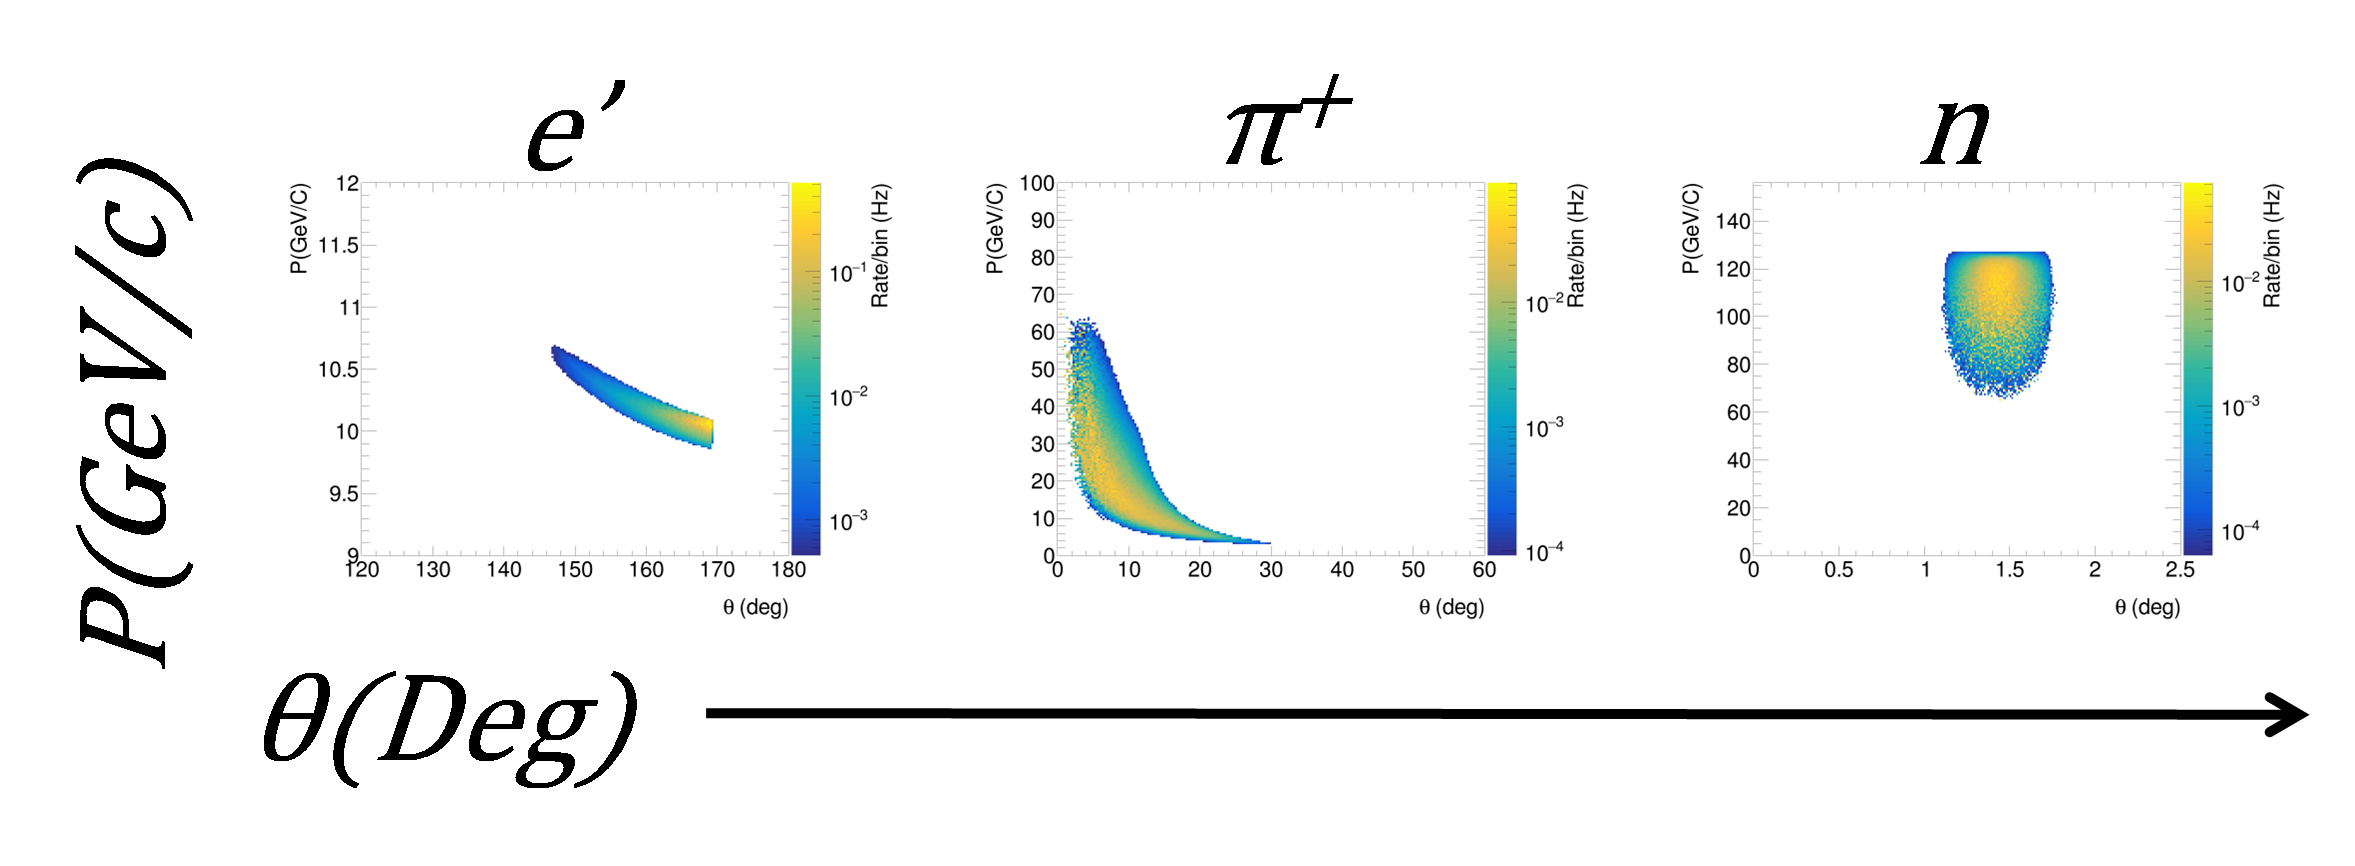
\includegraphics[width=\textwidth]{Figures/10on130_PiDEMP_Truth.png}
    \caption{Momentum and polar angle ($\theta$ distribution of scattered electrons, $e'$, pions, $\pi^{+}$ and neutrons, $n$ for 10x130 events. Note that the $z$ scale is a rate in $Hz$ due to the absolute normalisation of DEMPgen.}
\label{fig:10x130_TruthKin}
\end{figure}
\begin{figure}[h]
    \centering
    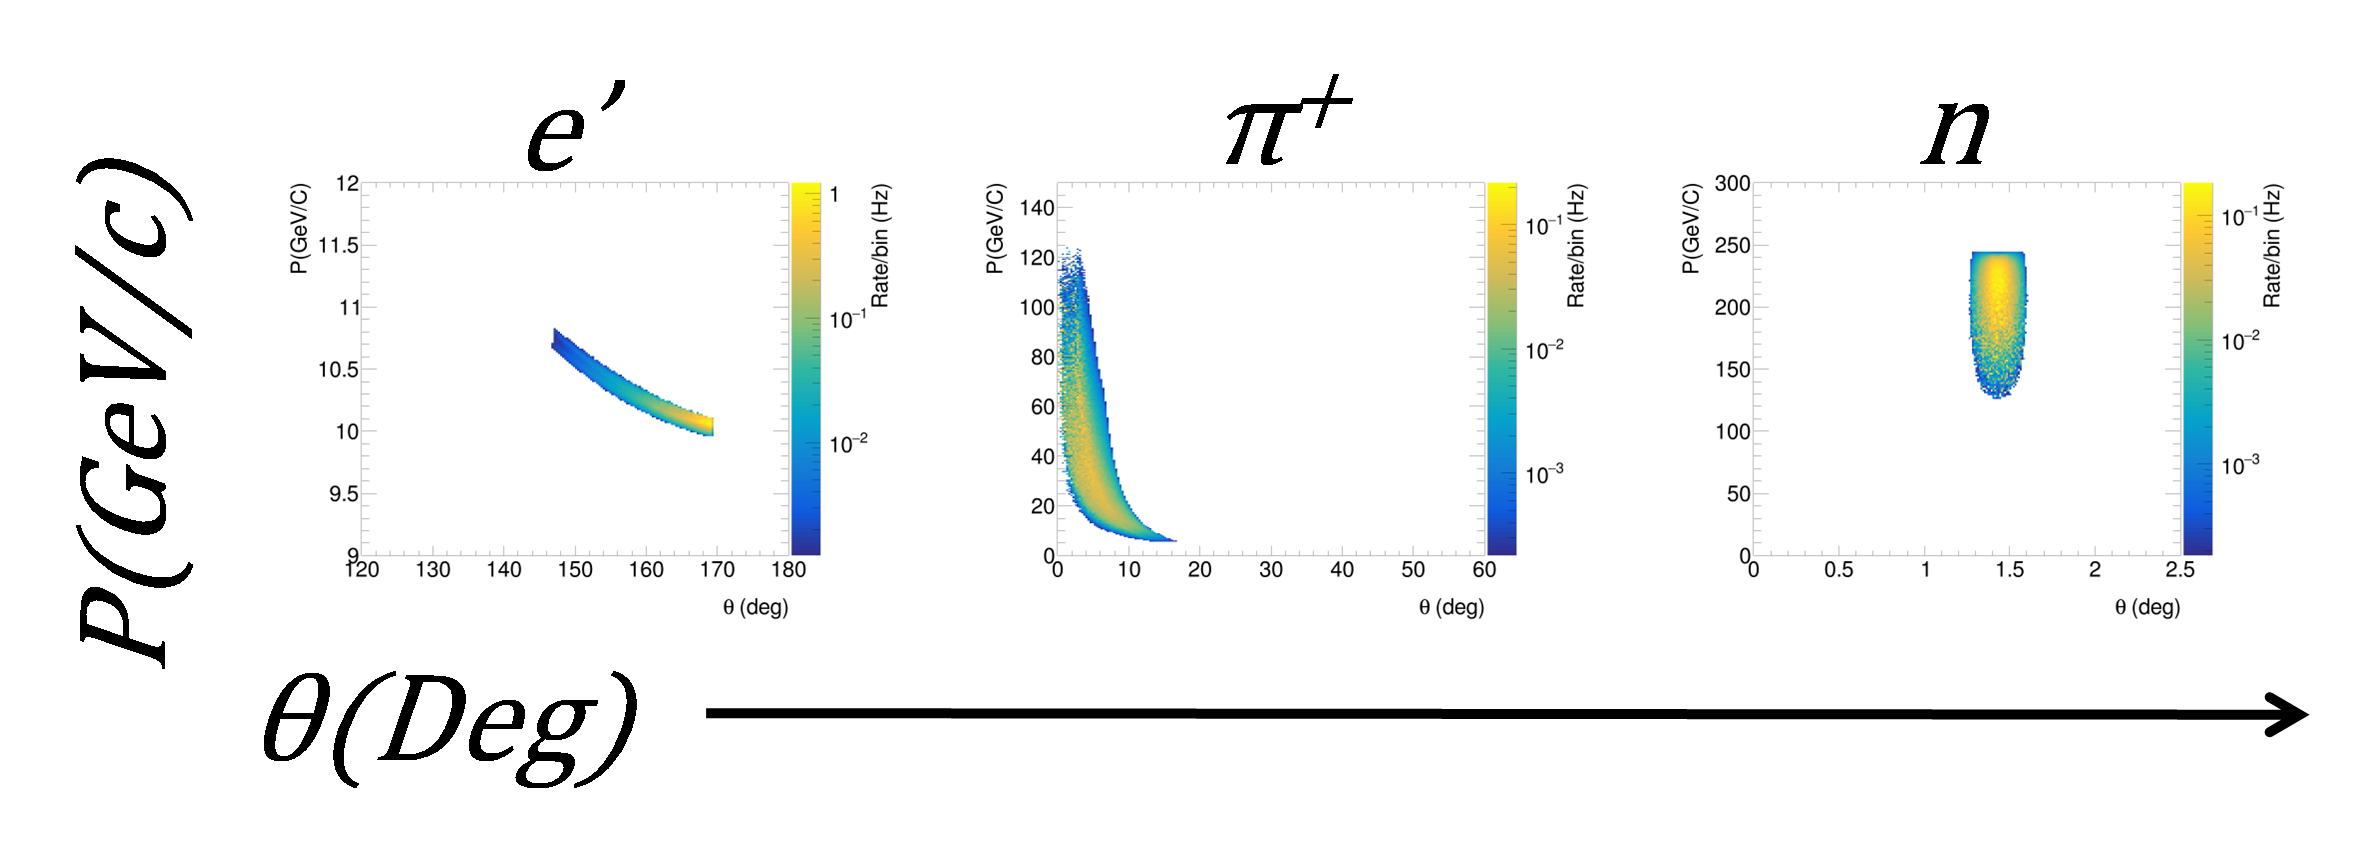
\includegraphics[width=\textwidth]{Figures/10on250_PiDEMP_Truth.png}
    \caption{Momentum and polar angle ($\theta$ distribution of scattered electrons, $e'$, pions, $\pi^{+}$ and neutrons, $n$ for 10x250 events. Note that the $z$ scale is a rate in $Hz$ due to the absolute normalisation of DEMPgen.}
\label{fig:10x250_TruthKin}
\end{figure}

This makes the event selection process relatively straightforward with a clearly defined sequence:

\begin{enumerate}
    \item Identify charged particles ($e'$ and $\pi^{+}$)
    \item Identify neutrons incident on the ZDC
    \item Calculate kinematics
    \item Apply exclusivity and other cuts
\end{enumerate}

Each stage has some cuts applied which are detailed below.

\subsection{Event Selection - Identifying Charged Particles}\label{subsec:Charged_Parts}

Due to the distribution of particles in DEMP $p(e,e'\pi^+n)$ events, selection of charged particles are very straightforward. \textcolor{red}{Change this to the electron finder when implemented! SJDK 21/07/25}. The electron is identified by selecting a reconstructed charged particle track (i.e. within the ``ReconstructedChargedParticles'' branch of the EICrecon output) with a negative charge, with the track momentum in the $-z$ direction. There is also a requirement that this track has $\lvert \vec{P} \rvert$ greater than $80\%$ of the incident electron beam energy, $8~GeV/c$ in both beam energy combinations studied in this note. 

The pion is identified by selecting a reconstructed charged particle track with a positive charge and with the track momentum in the $+z$ direction. There is also a requirement that this track has $\lvert \vec{P} \rvert$ greater than $1~GeV/c$. This requirement is included to remove any low momentum noise/background events that may be present.

\subsection{Event Selection - Identifying Neutrons}\label{subsec:Neutrons}

For the beam energy combinations studied, the neutron produced in this reaction is incident on, and detected in, the ZDC in almost all generated events. As such, neutron identification is straightforward. Neutrons are identified from the ``ReconstructedFarForwardZDCNeutrals'' EICrecon branch. To filter out events that are not incident upon the ZDC and to remove low energy events, cuts are implemented on $\theta^{*}$ and the reconstructed neutral particle energy. $\theta^{*}$ is the polar angle $\theta$ after a rotation of $25~mRad$ around the proton beam axis to remove the effect of the beam crossing angle. After this rotation, the ZDC is indeed, centred at roughly ``zero degrees''. A cut of $\theta^{*}<4~mRad$ is applied. To remove low energy hits, a cut-off of the neutral particle energy being greater than $40~GeV$ is applied for 10x130 events. For 10x250 events, this cut off is increased to $120~GeV$.

\subsection{Event Selection - Calculate Kinematics}\label{subsec:Kinematic_Calcs}

Before calculating any kinematic quantities such as $Q^{2}$ and $-t$, the analysis code requires that a candidate $e'$, $\pi^{+}$ and $n$ that pass relevant selection cuts (as defined above) have been found in coincidence. If this condition is met, the code calculates $Q^{2}$, the negative four-momentum transfer squared at the electron vertex. $Q^{2}$ can be calculated using various different methods as discussed \href{https://agenda.infn.it/event/43344/contributions/253198/attachments/130672/194493/EIC_KinematicReconstruction.pdf}{here}\footnote{\url{https://agenda.infn.it/event/43344/contributions/253198/attachments/130672/194493/EIC_KinematicReconstruction.pdf}}. For the kinematic region under investigation in this study, the double angle, DA, method proved to be optimal as seen in Fig~.\ref{fig:Q2_Comp}. It is apparent that this calculation method closely matches the ``true'' value across the relevant $Q^{2}$ range (5 to 35) as seen in Fig.~\ref{fig:Q2DA_Comp}. Once calculated, a cut on $Q^{2}_{DA}$ being within 5 and 35 $(GeV/c)^{2}$ is applied.

\begin{figure}[h]
    \centering
    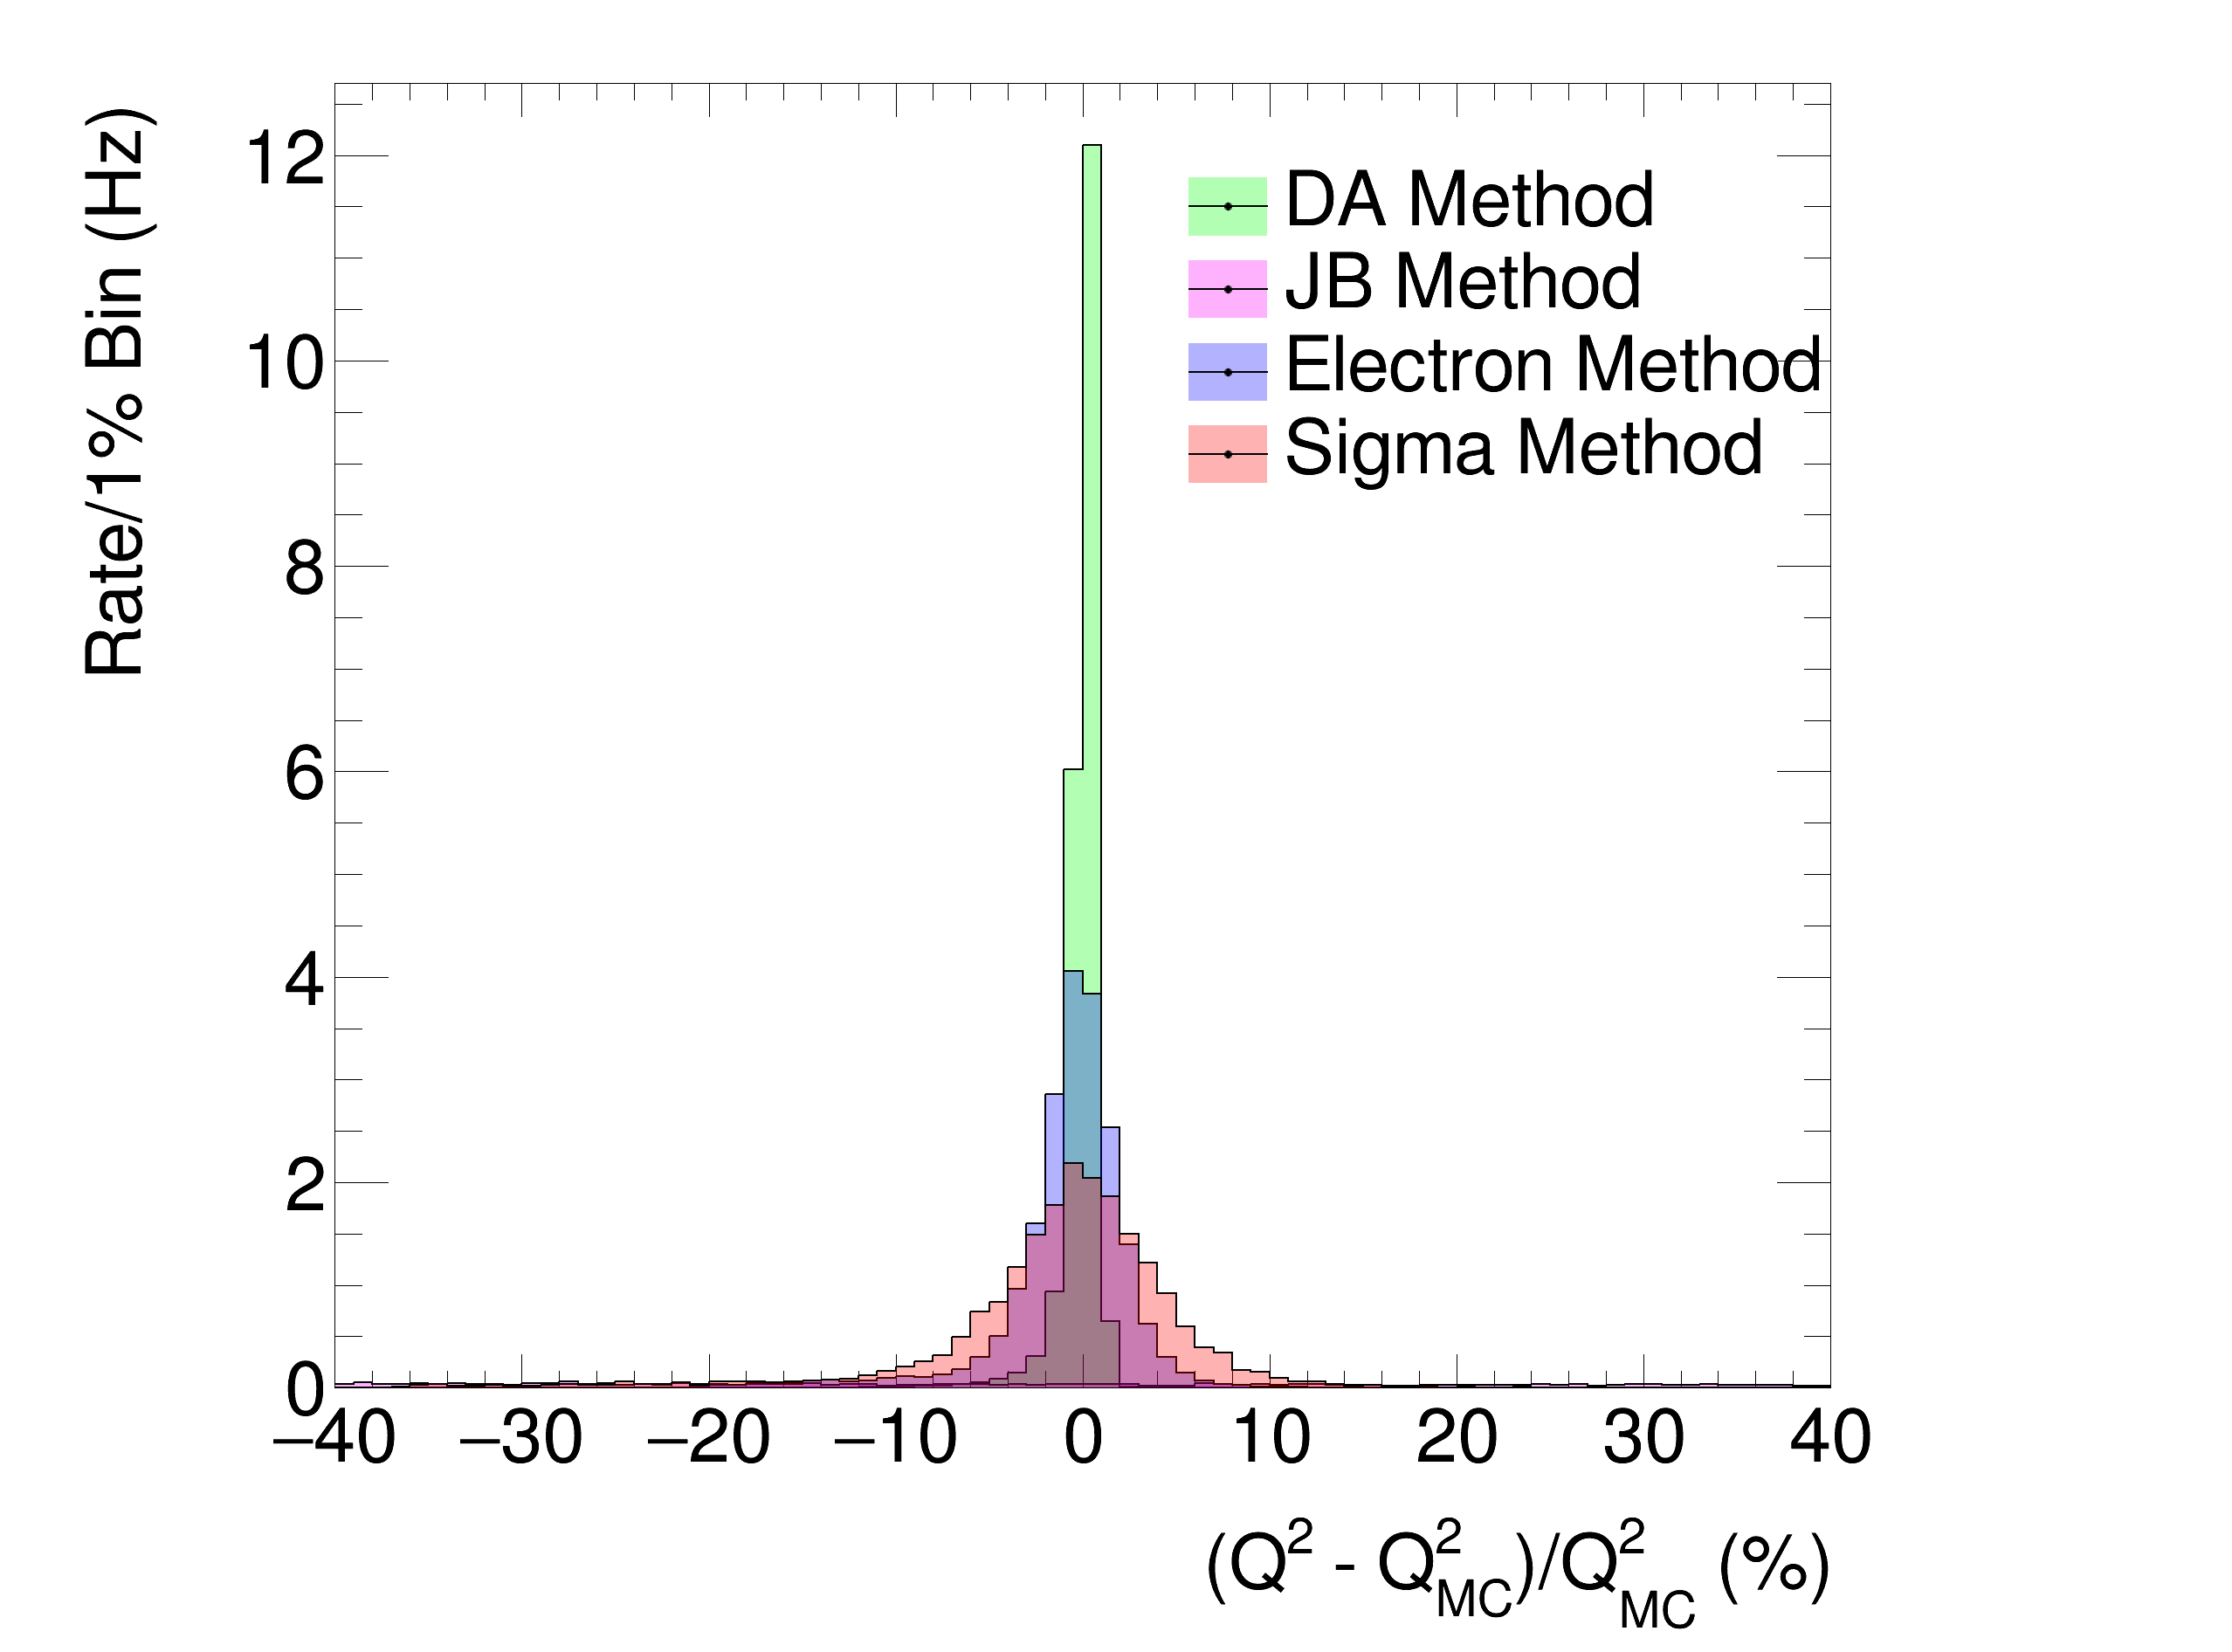
\includegraphics[width=0.475\textwidth]{Figures/10on130_Q2Comp.png}
    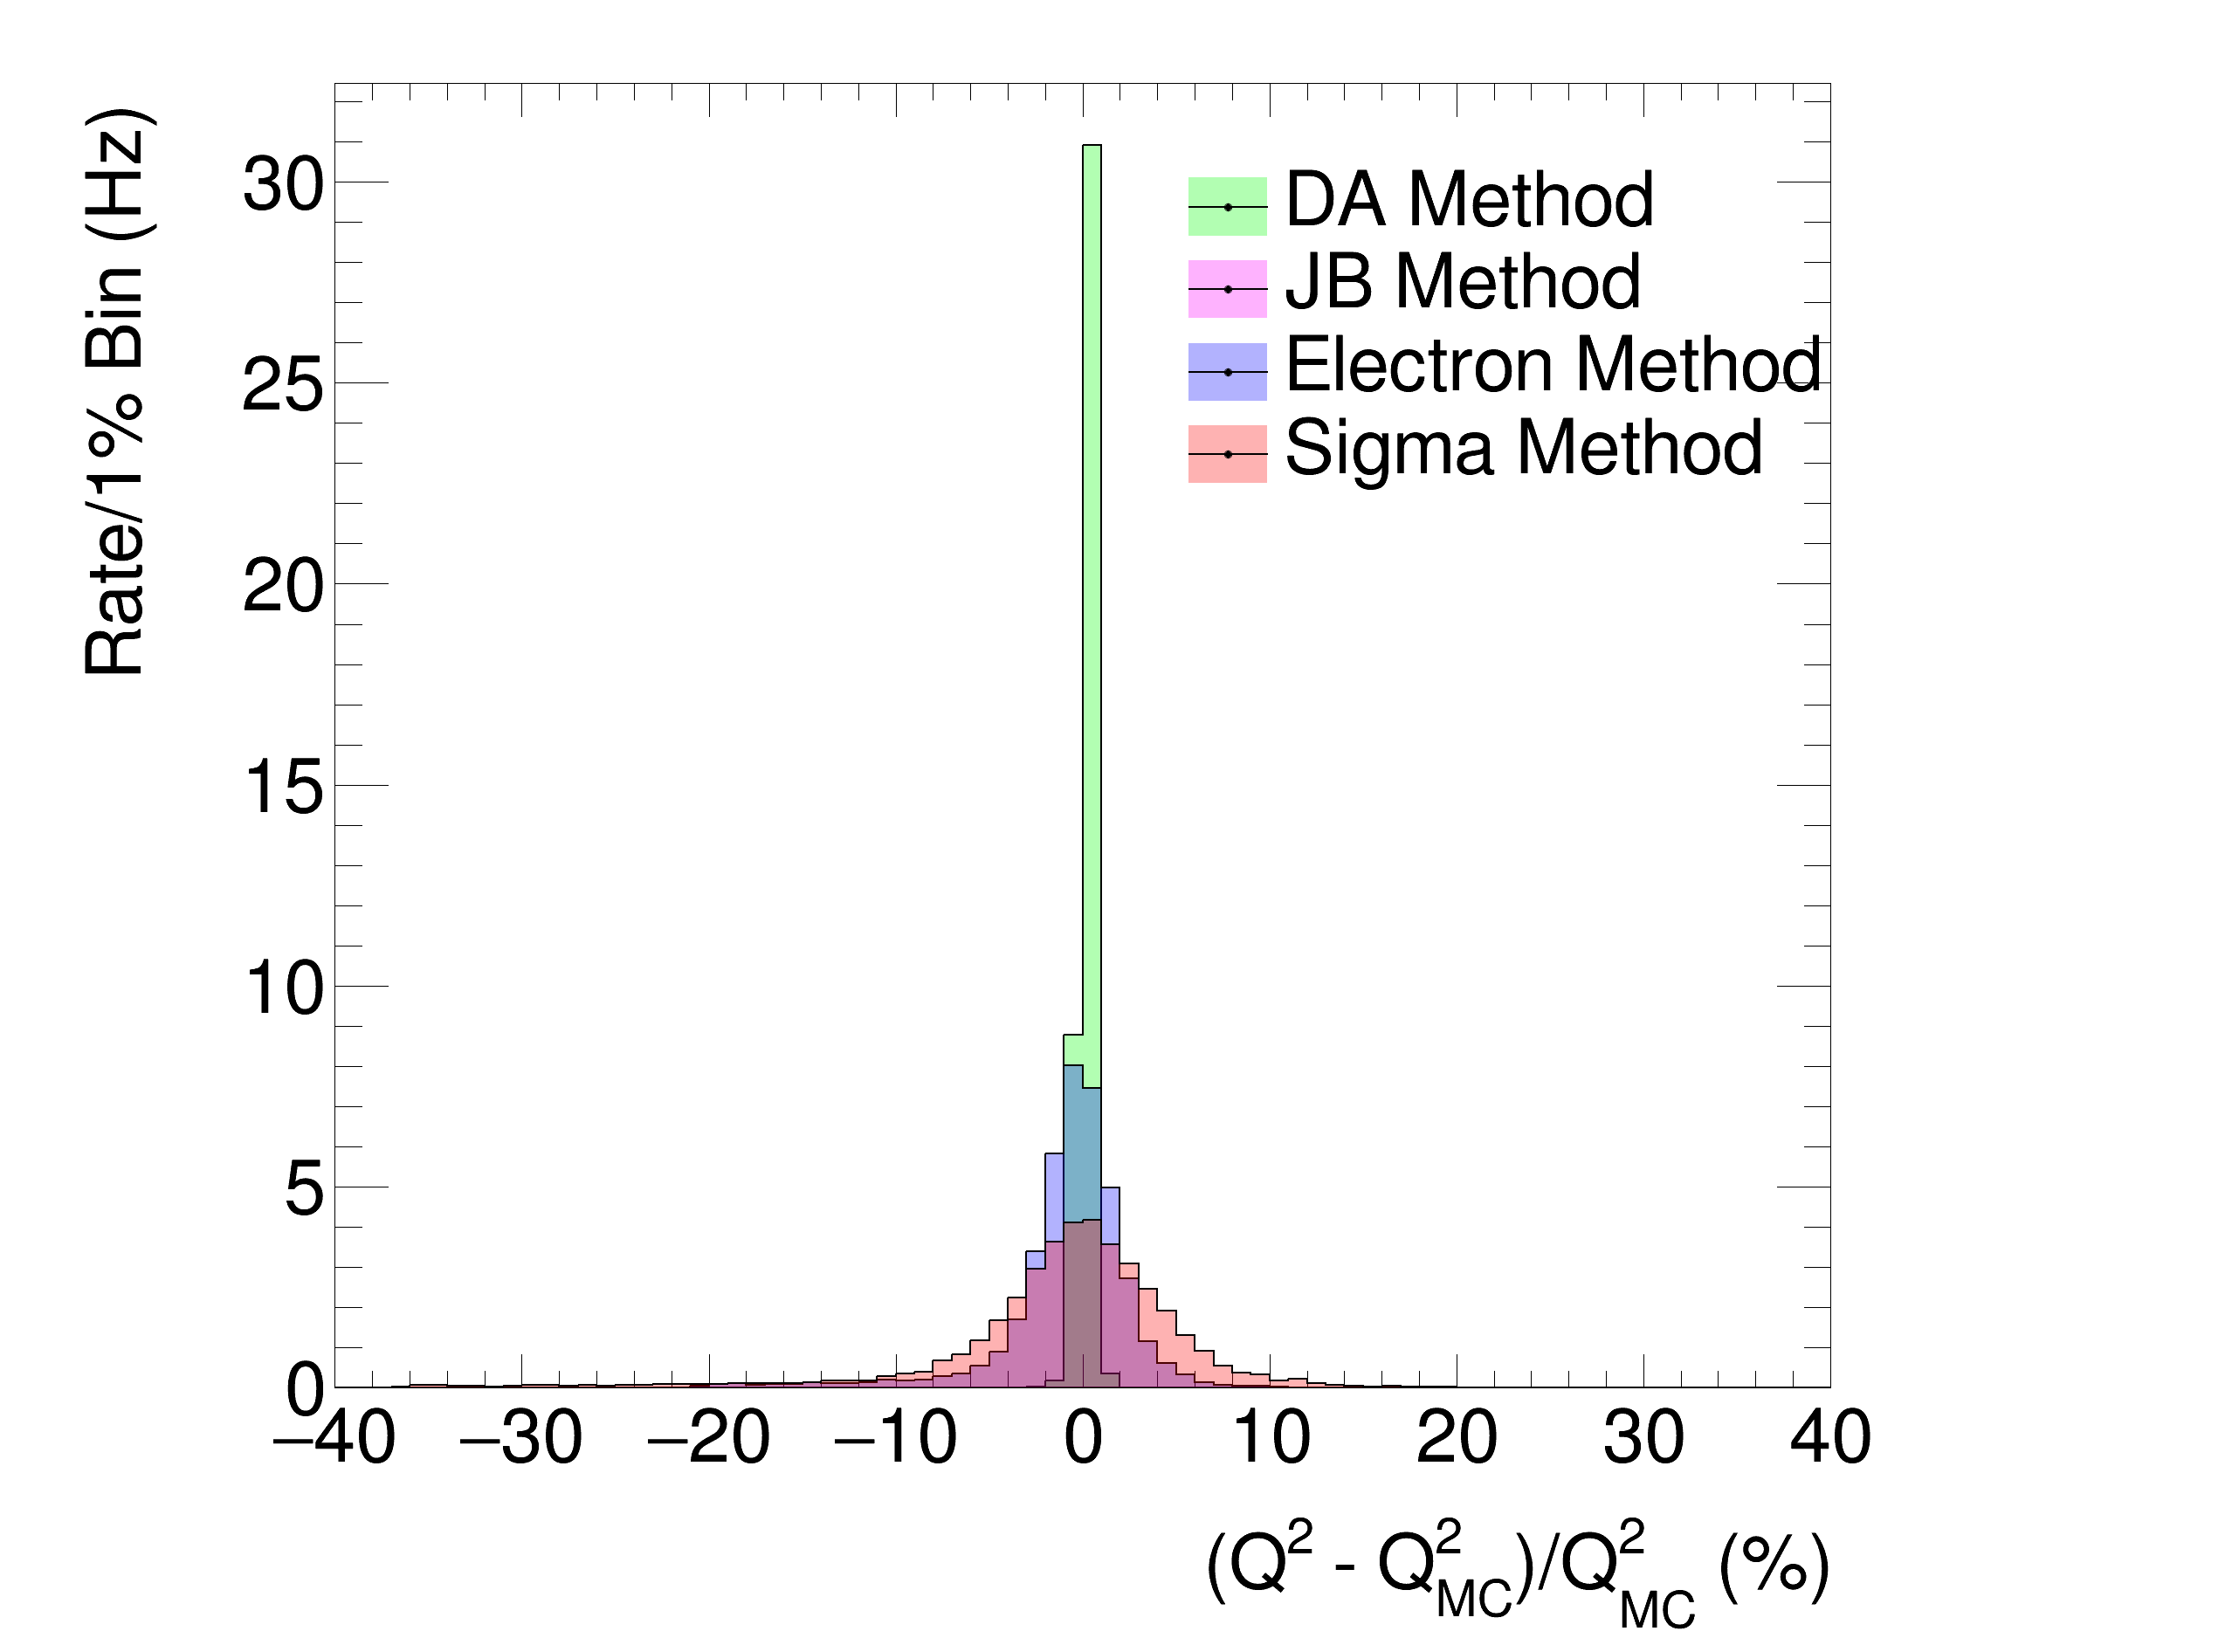
\includegraphics[width=0.475\textwidth]{Figures/10on250_Q2Comp.png}
    \caption{A comparison of the resolution for calculated $Q^{2}$ values, defined as the deviation from the MC truth divided by the MC truth value and expressed as a percentage, for 10x130 (left) and 10x250 (right) event samples. $Q^{2}_{DA}$ is clearly the most accurate in both cases, note that it is clear that the JB method is not applicable in DEMP kinematics. The distribution for this extends beyond the range of the plot quite significantly.}
\label{fig:Q2_Comp}
\end{figure}

\begin{figure}[h]
    \centering
    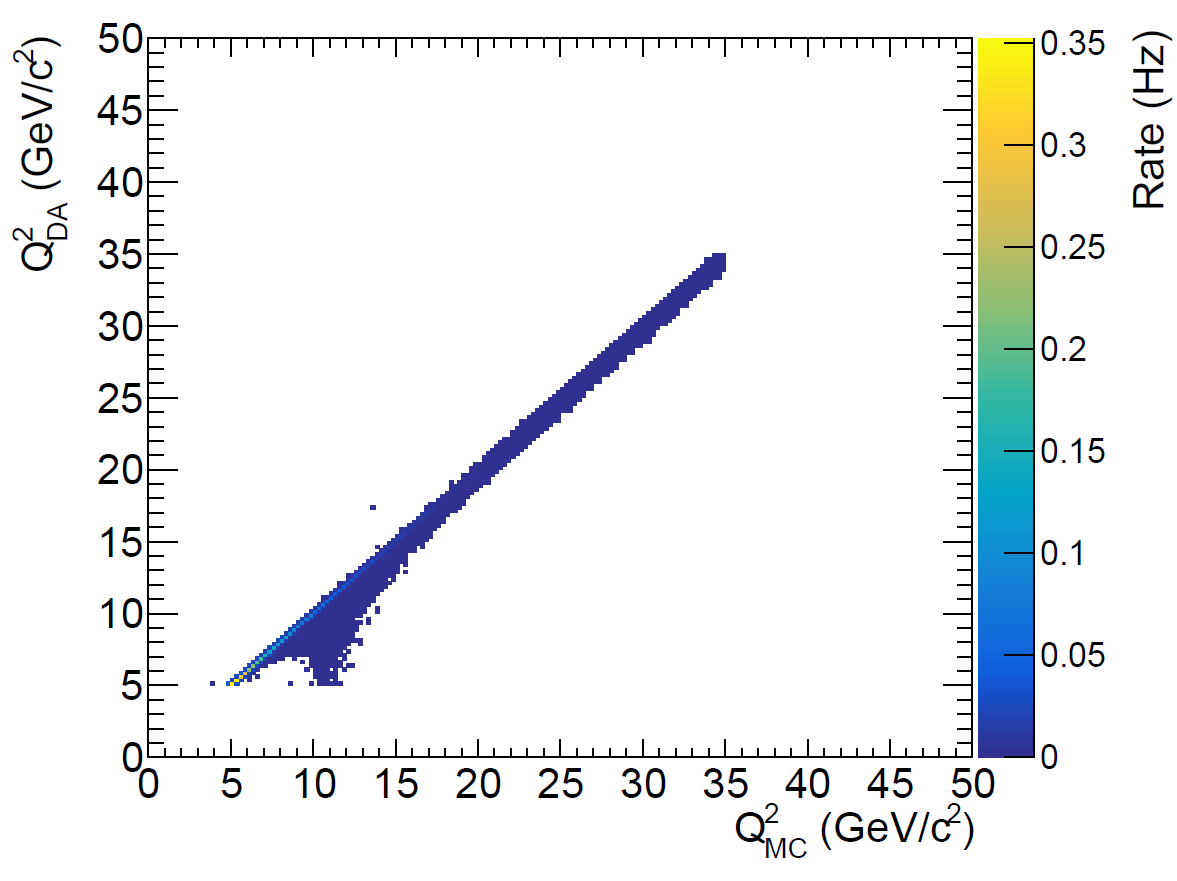
\includegraphics[width=0.475\textwidth]{Figures/10on130_Q2DAComp.png}
    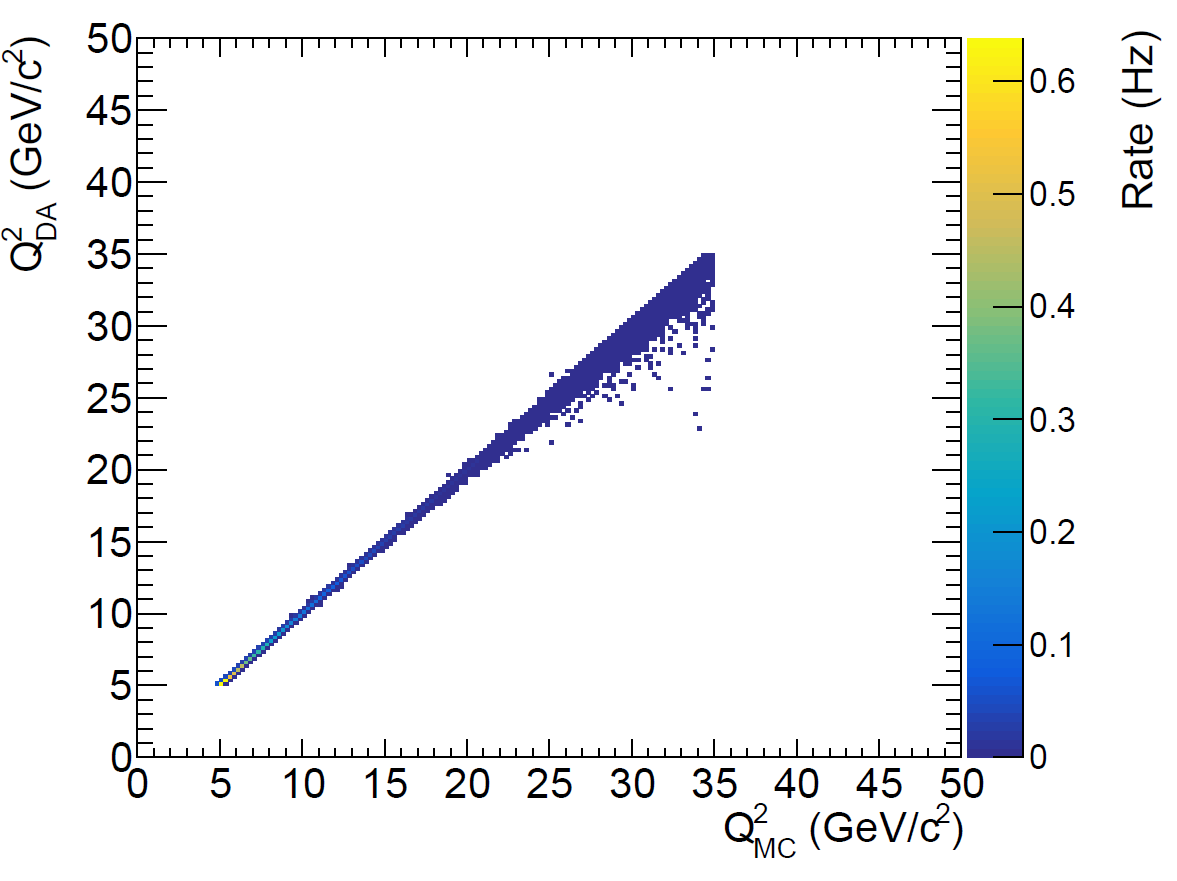
\includegraphics[width=0.475\textwidth]{Figures/10on250_Q2DAComp.png}
    \caption{A comparison of $Q^{2}_{DA}$ against the MC truth value of $Q^{2}$ for 10x130 (left) and 10x250 (right) event samples.}
\label{fig:Q2DA_Comp}
\end{figure}

Once events outside the relevant $Q^{2}$ range are removed, further kinematic quantities are calculated. The squared four-momentum transfer between the initial ($p$) and final ($n$) hadron state, $-t$, is critical to determine accurately for DEMP studies. Measurements are needed at the lowest $-t$ possible in order to get as close to the pion pole as possible. As with $Q^{2}$, there are many ways to determine $-t$. These are defined in the $t$RECO convention document \textcolor{red}{need a link/reference/citation for this! If none, add relevant text for the calculation. Link to generic code etc.}. DEMP can utilise the $t_{eXBABE}$ method which exploits the exclusive nature of the reaction to ``correct'' the measured neutron track. This method outperforms any reconstruction methods as can be seen in Fig.~\ref{fig:t_Comp}. This determination of $-t$ also strongly correlates with the MC truth value of $-t$ as can be seen in Fig.~\ref{fig:teXBABE_Comp}.

\begin{figure}[h]
    \centering
    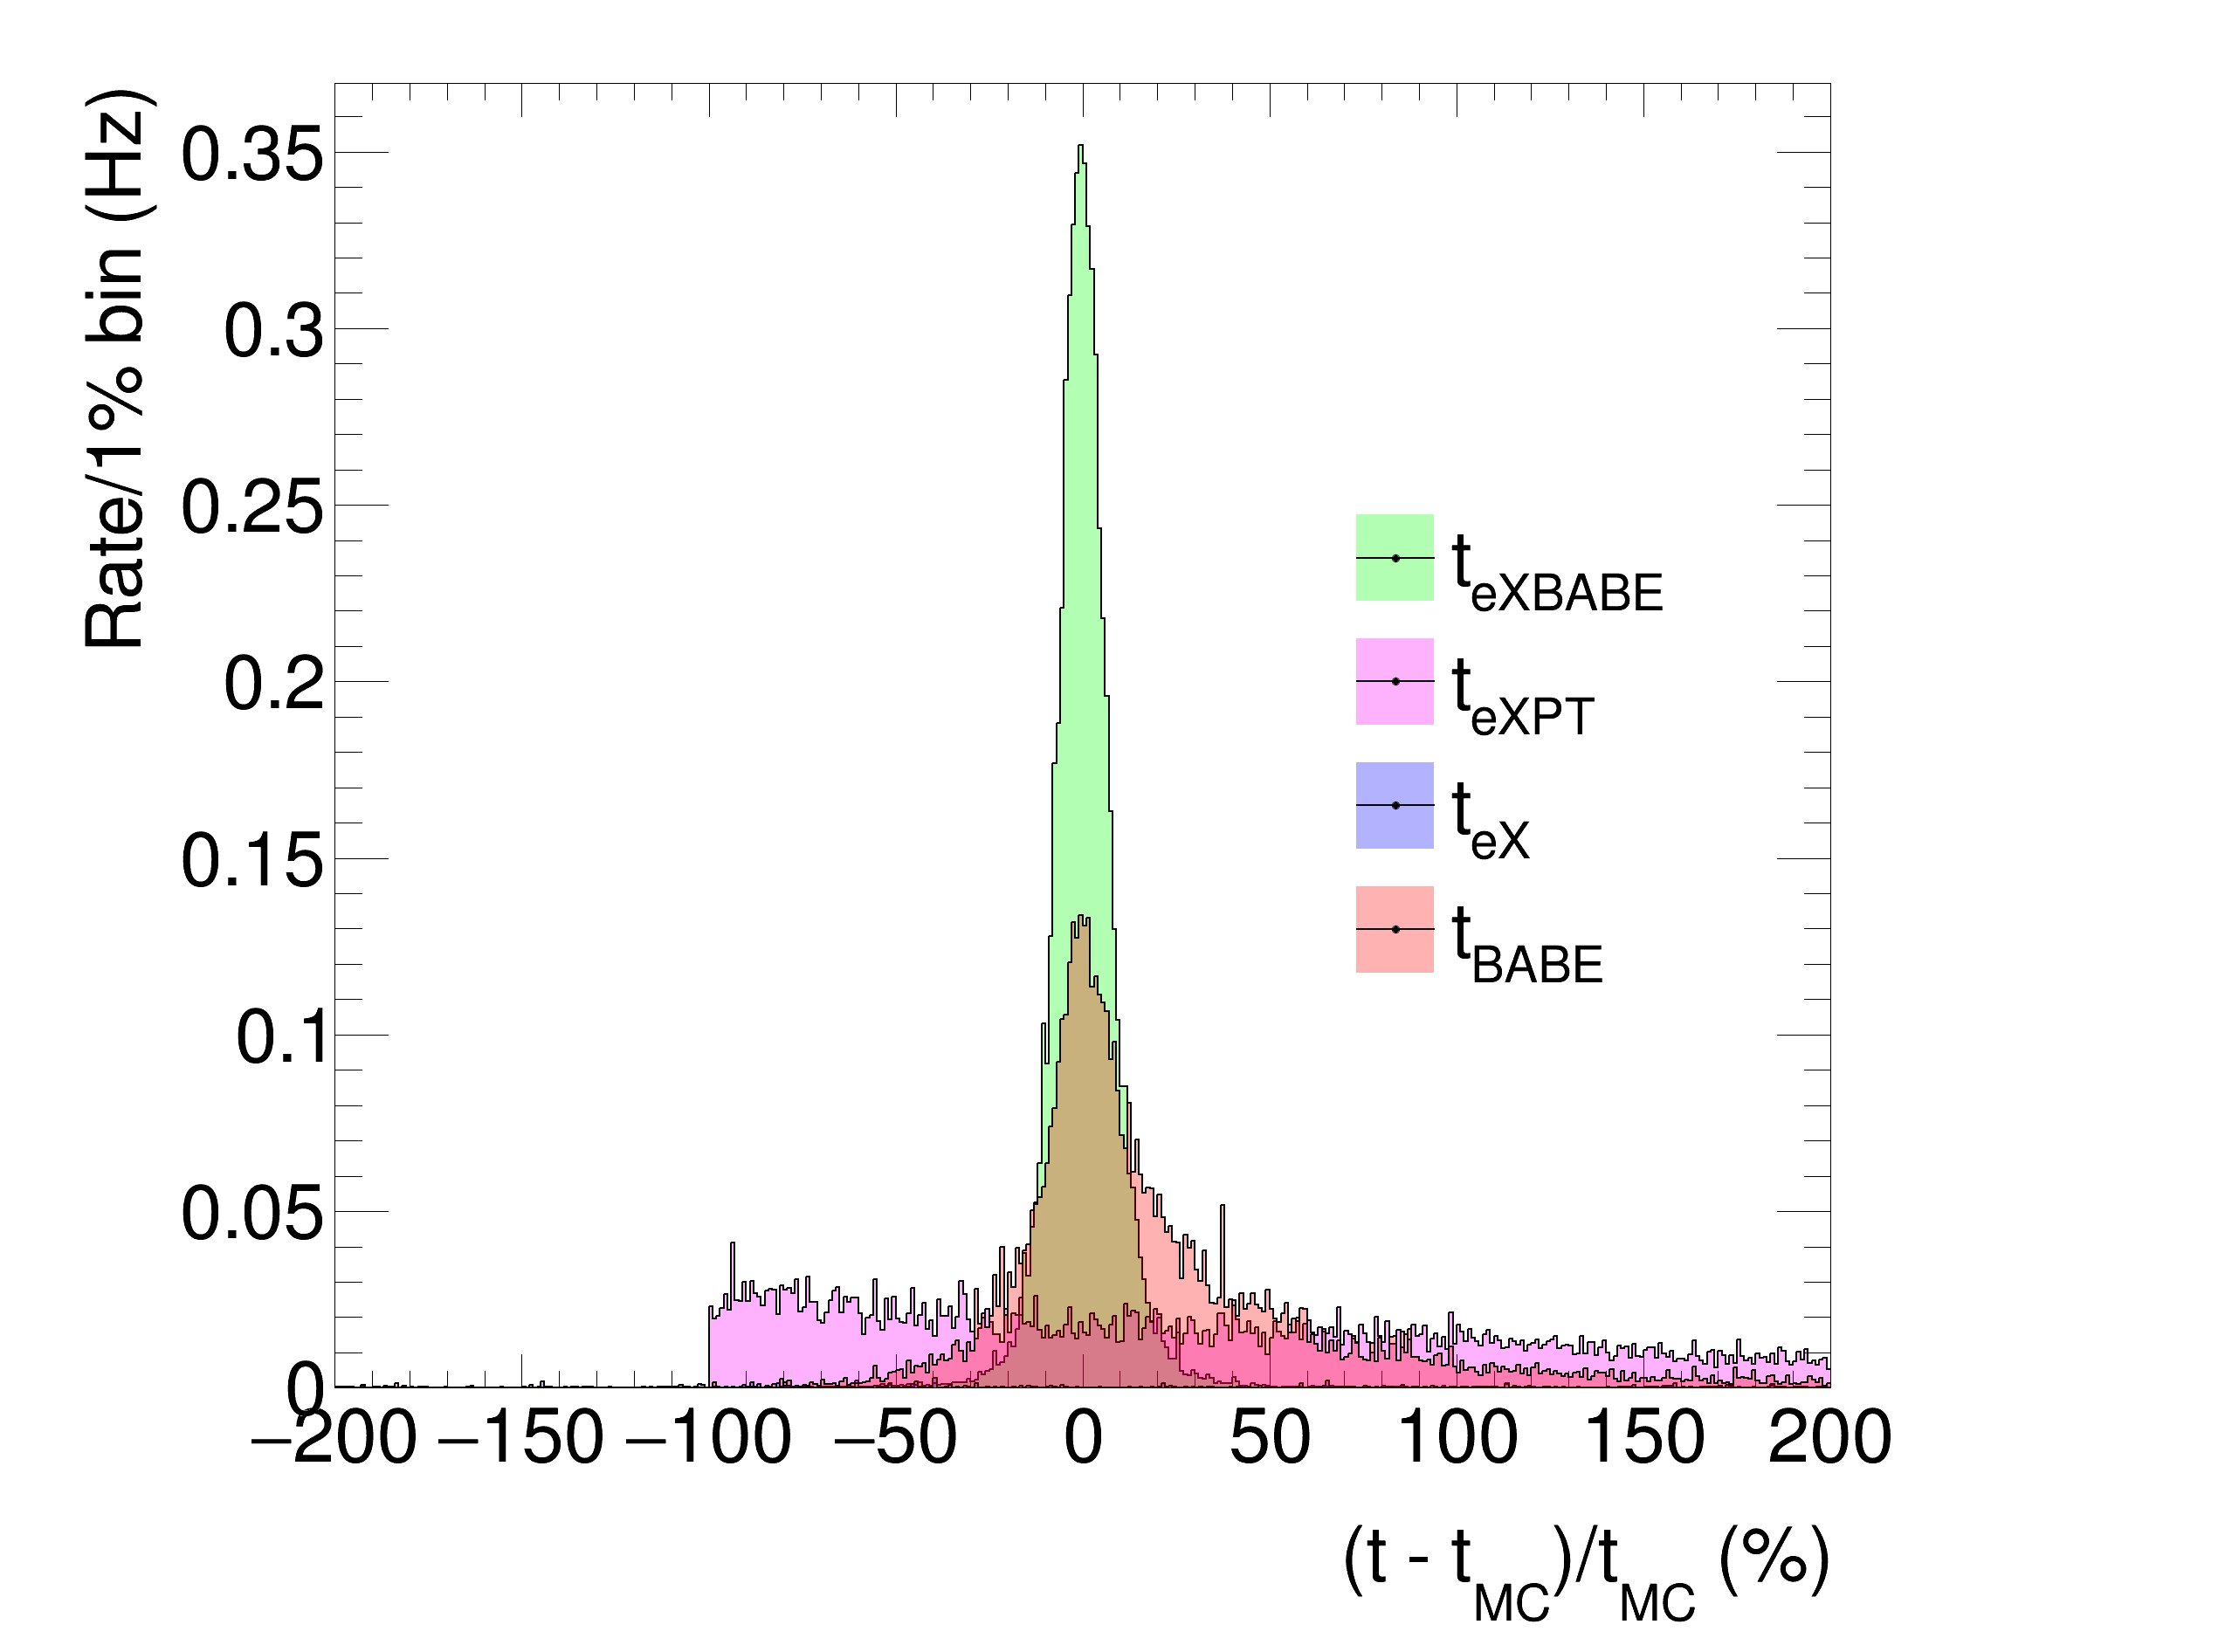
\includegraphics[width=0.475\textwidth]{Figures/10on130_tComp.png}
    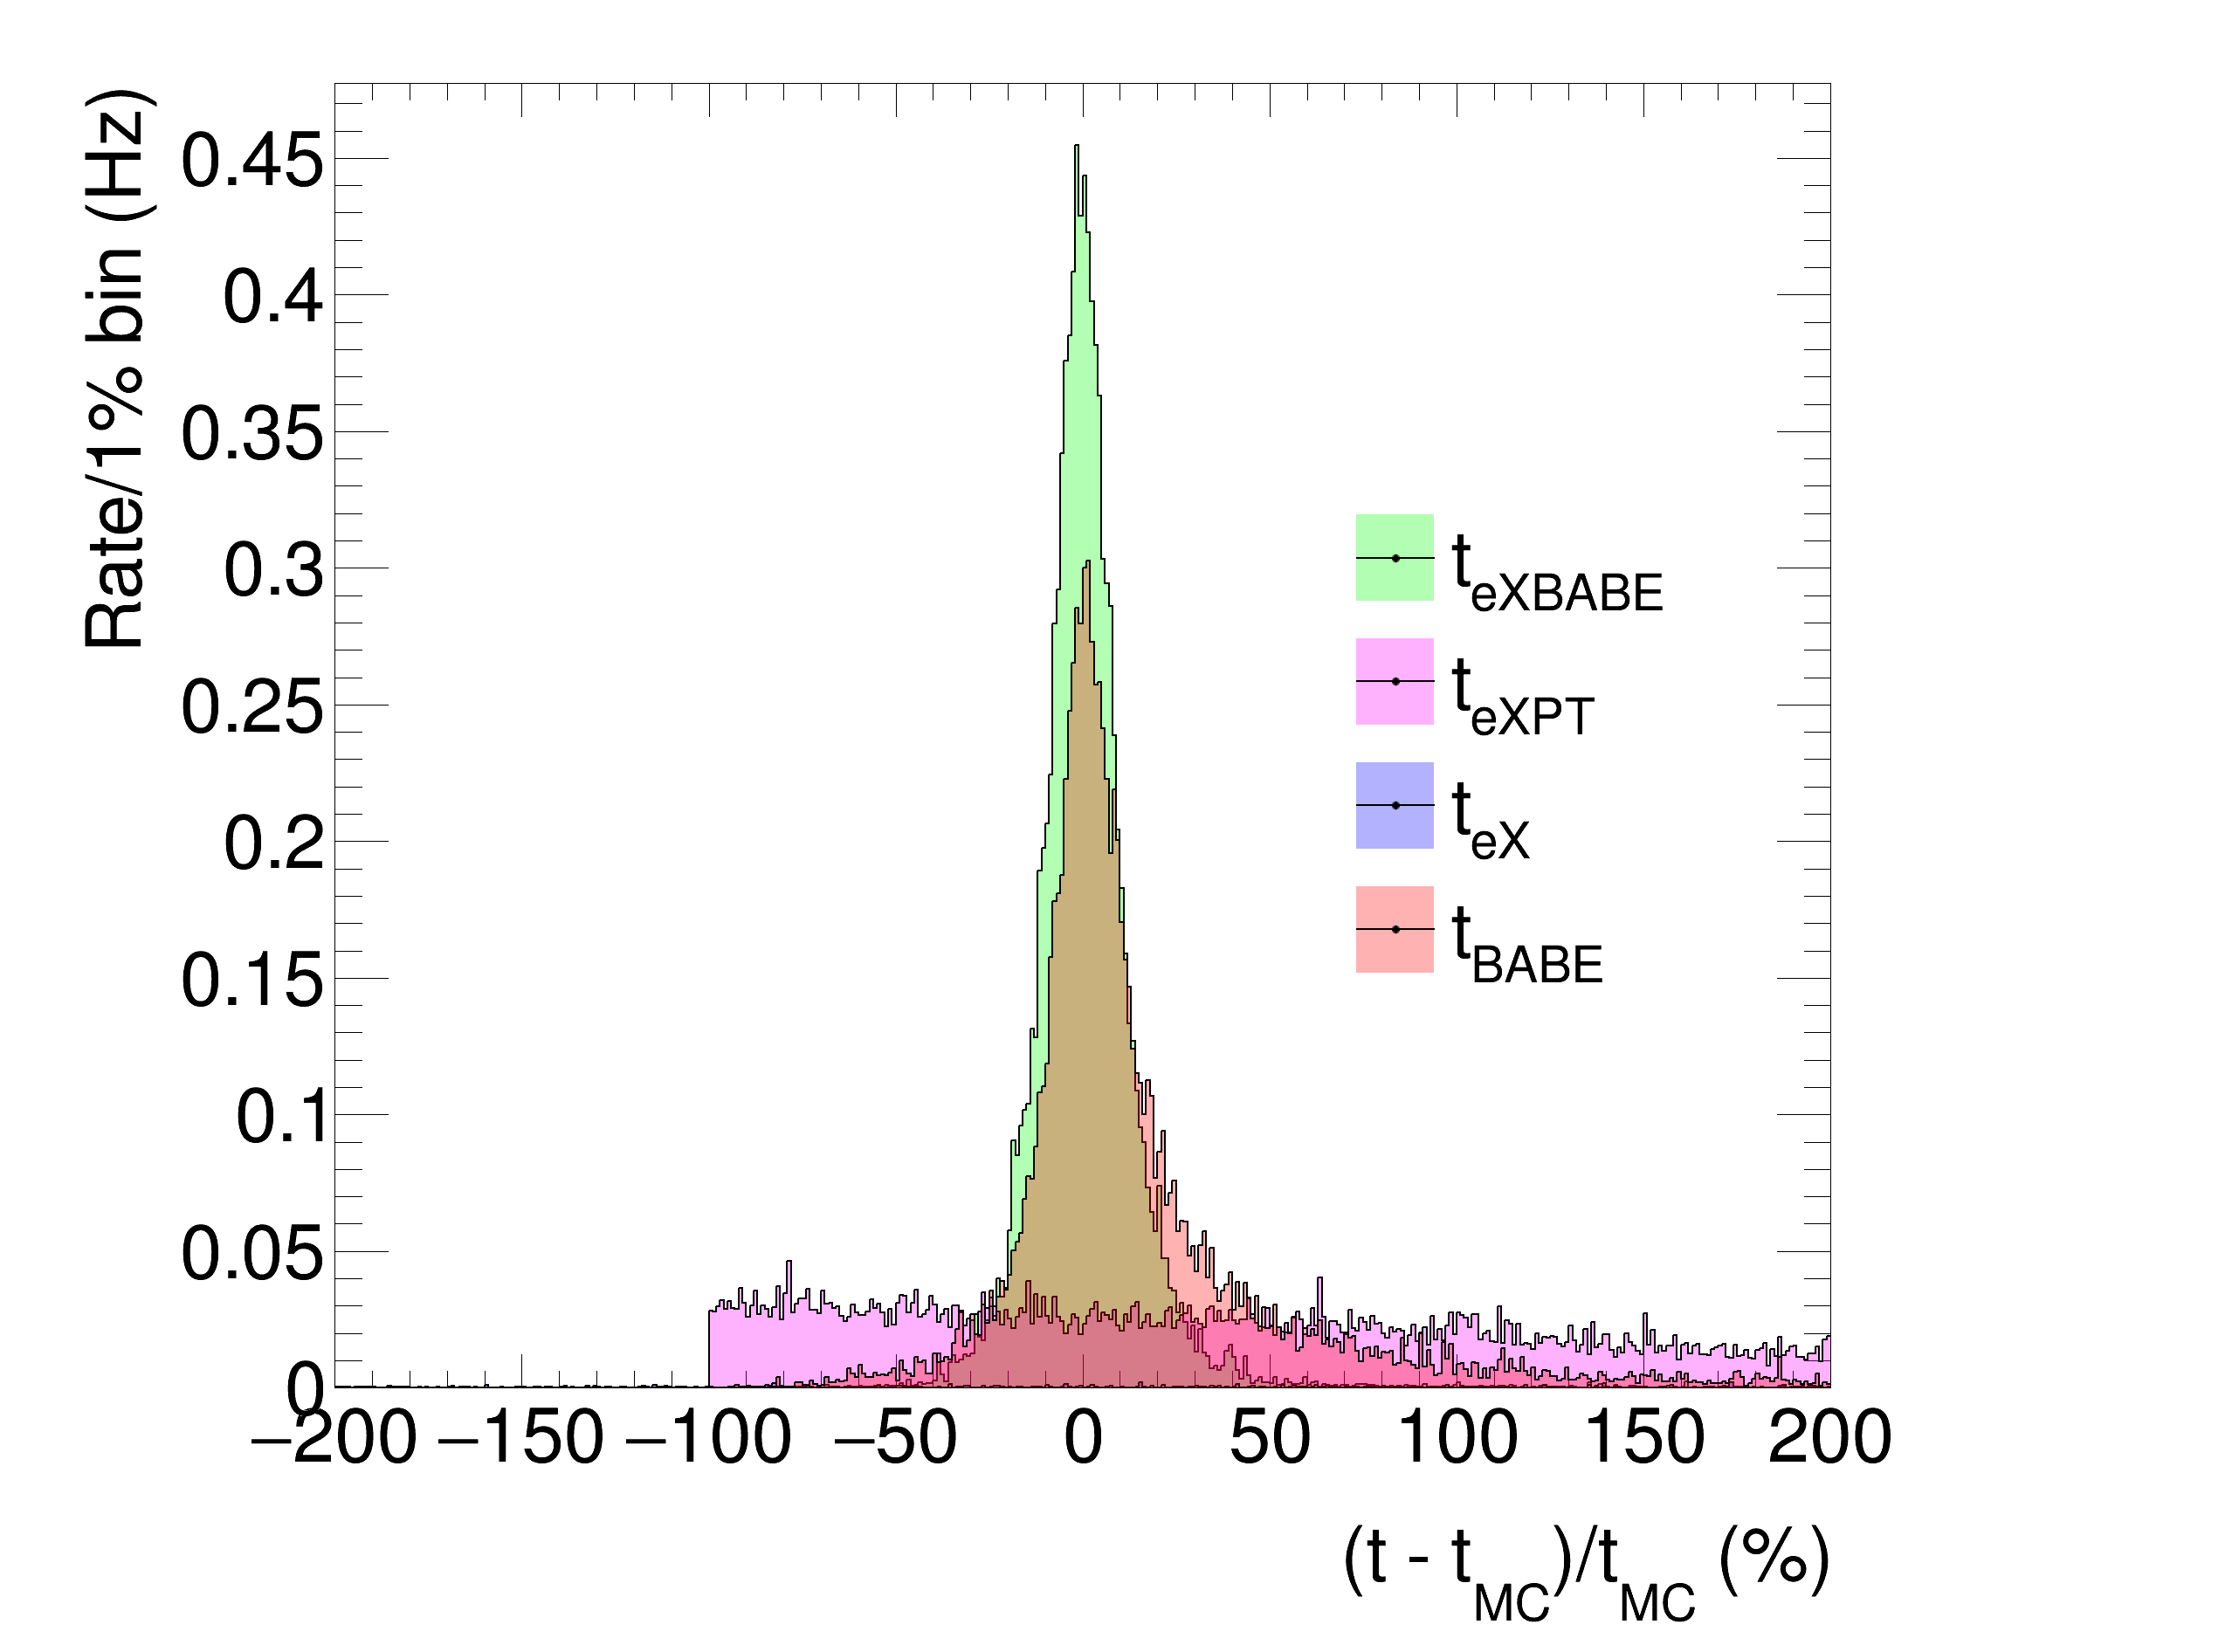
\includegraphics[width=0.475\textwidth]{Figures/10on250_tComp.png}
    \caption{A comparison of the resolution for calculated $-t$ values, defined as the deviation from the MC truth divided by the MC truth value and expressed as a percentage, for 10x130 (left) and 10x250 (right) event samples. $t_{eXBABE}$ is clearly the most accurate determination in each case.}
\label{fig:t_Comp}
\end{figure}

\begin{figure}[h]
    \centering
    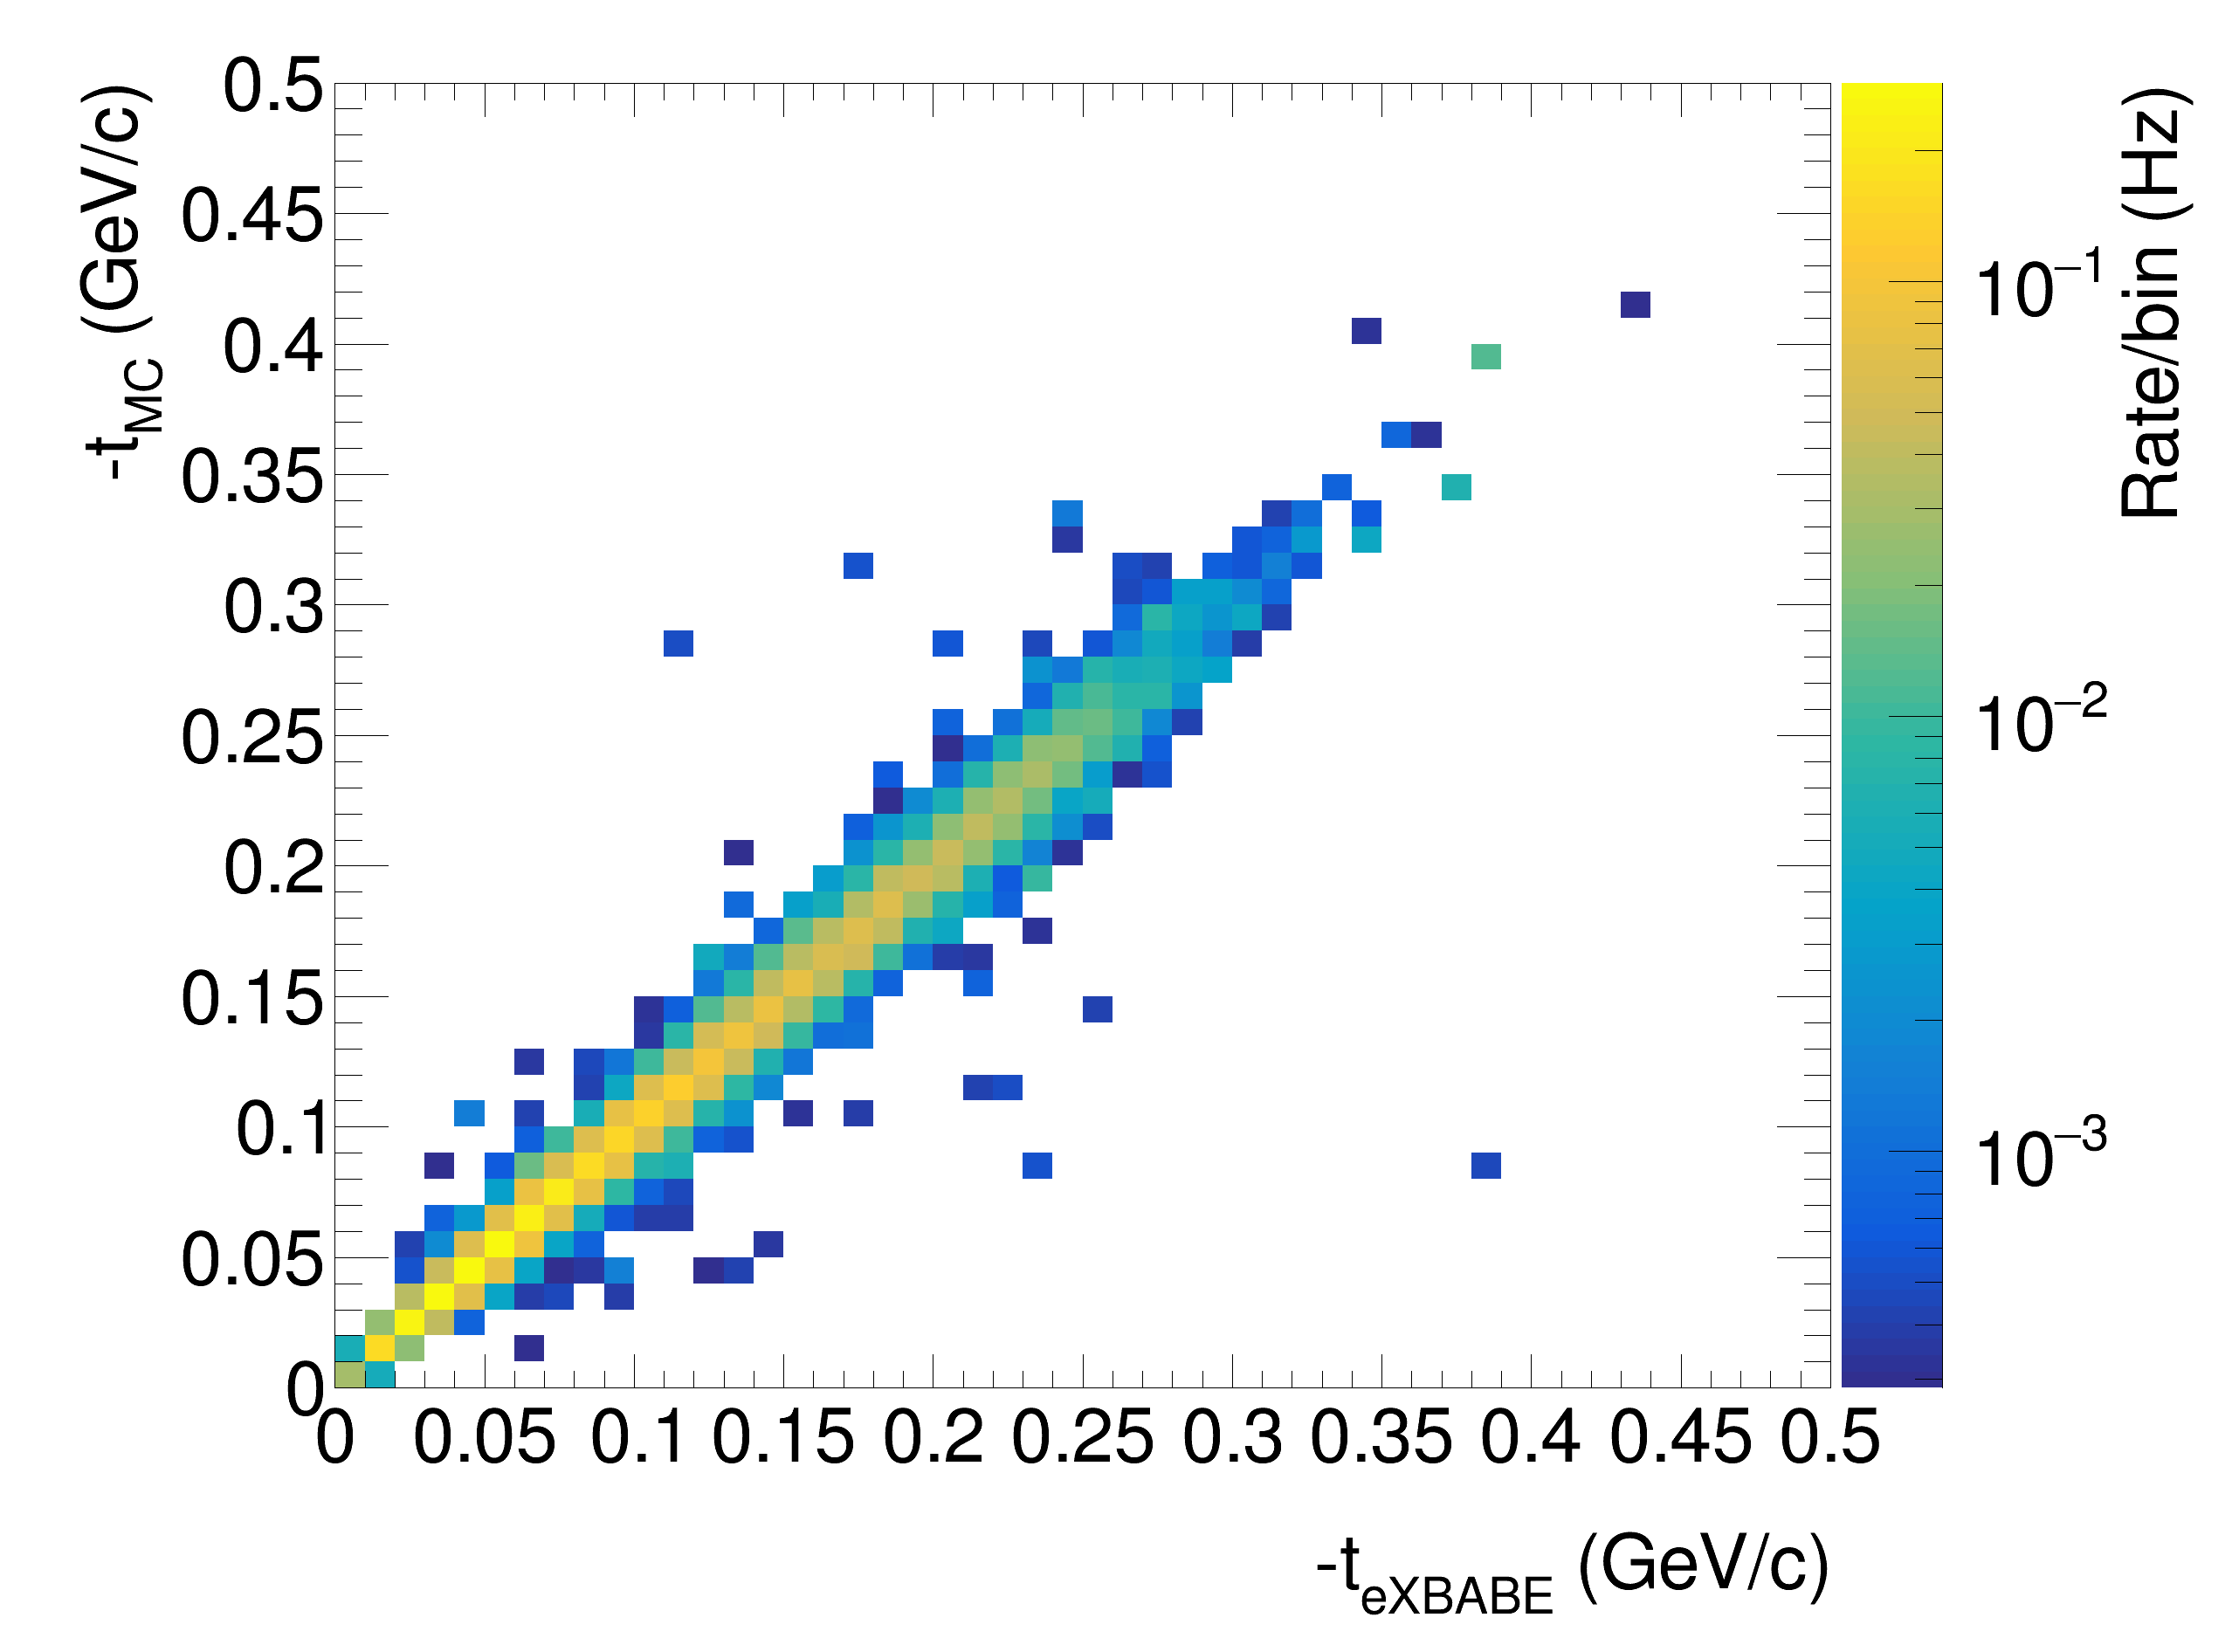
\includegraphics[width=0.475\textwidth]{Figures/10on130_tCompAlt_ZDC.png}
    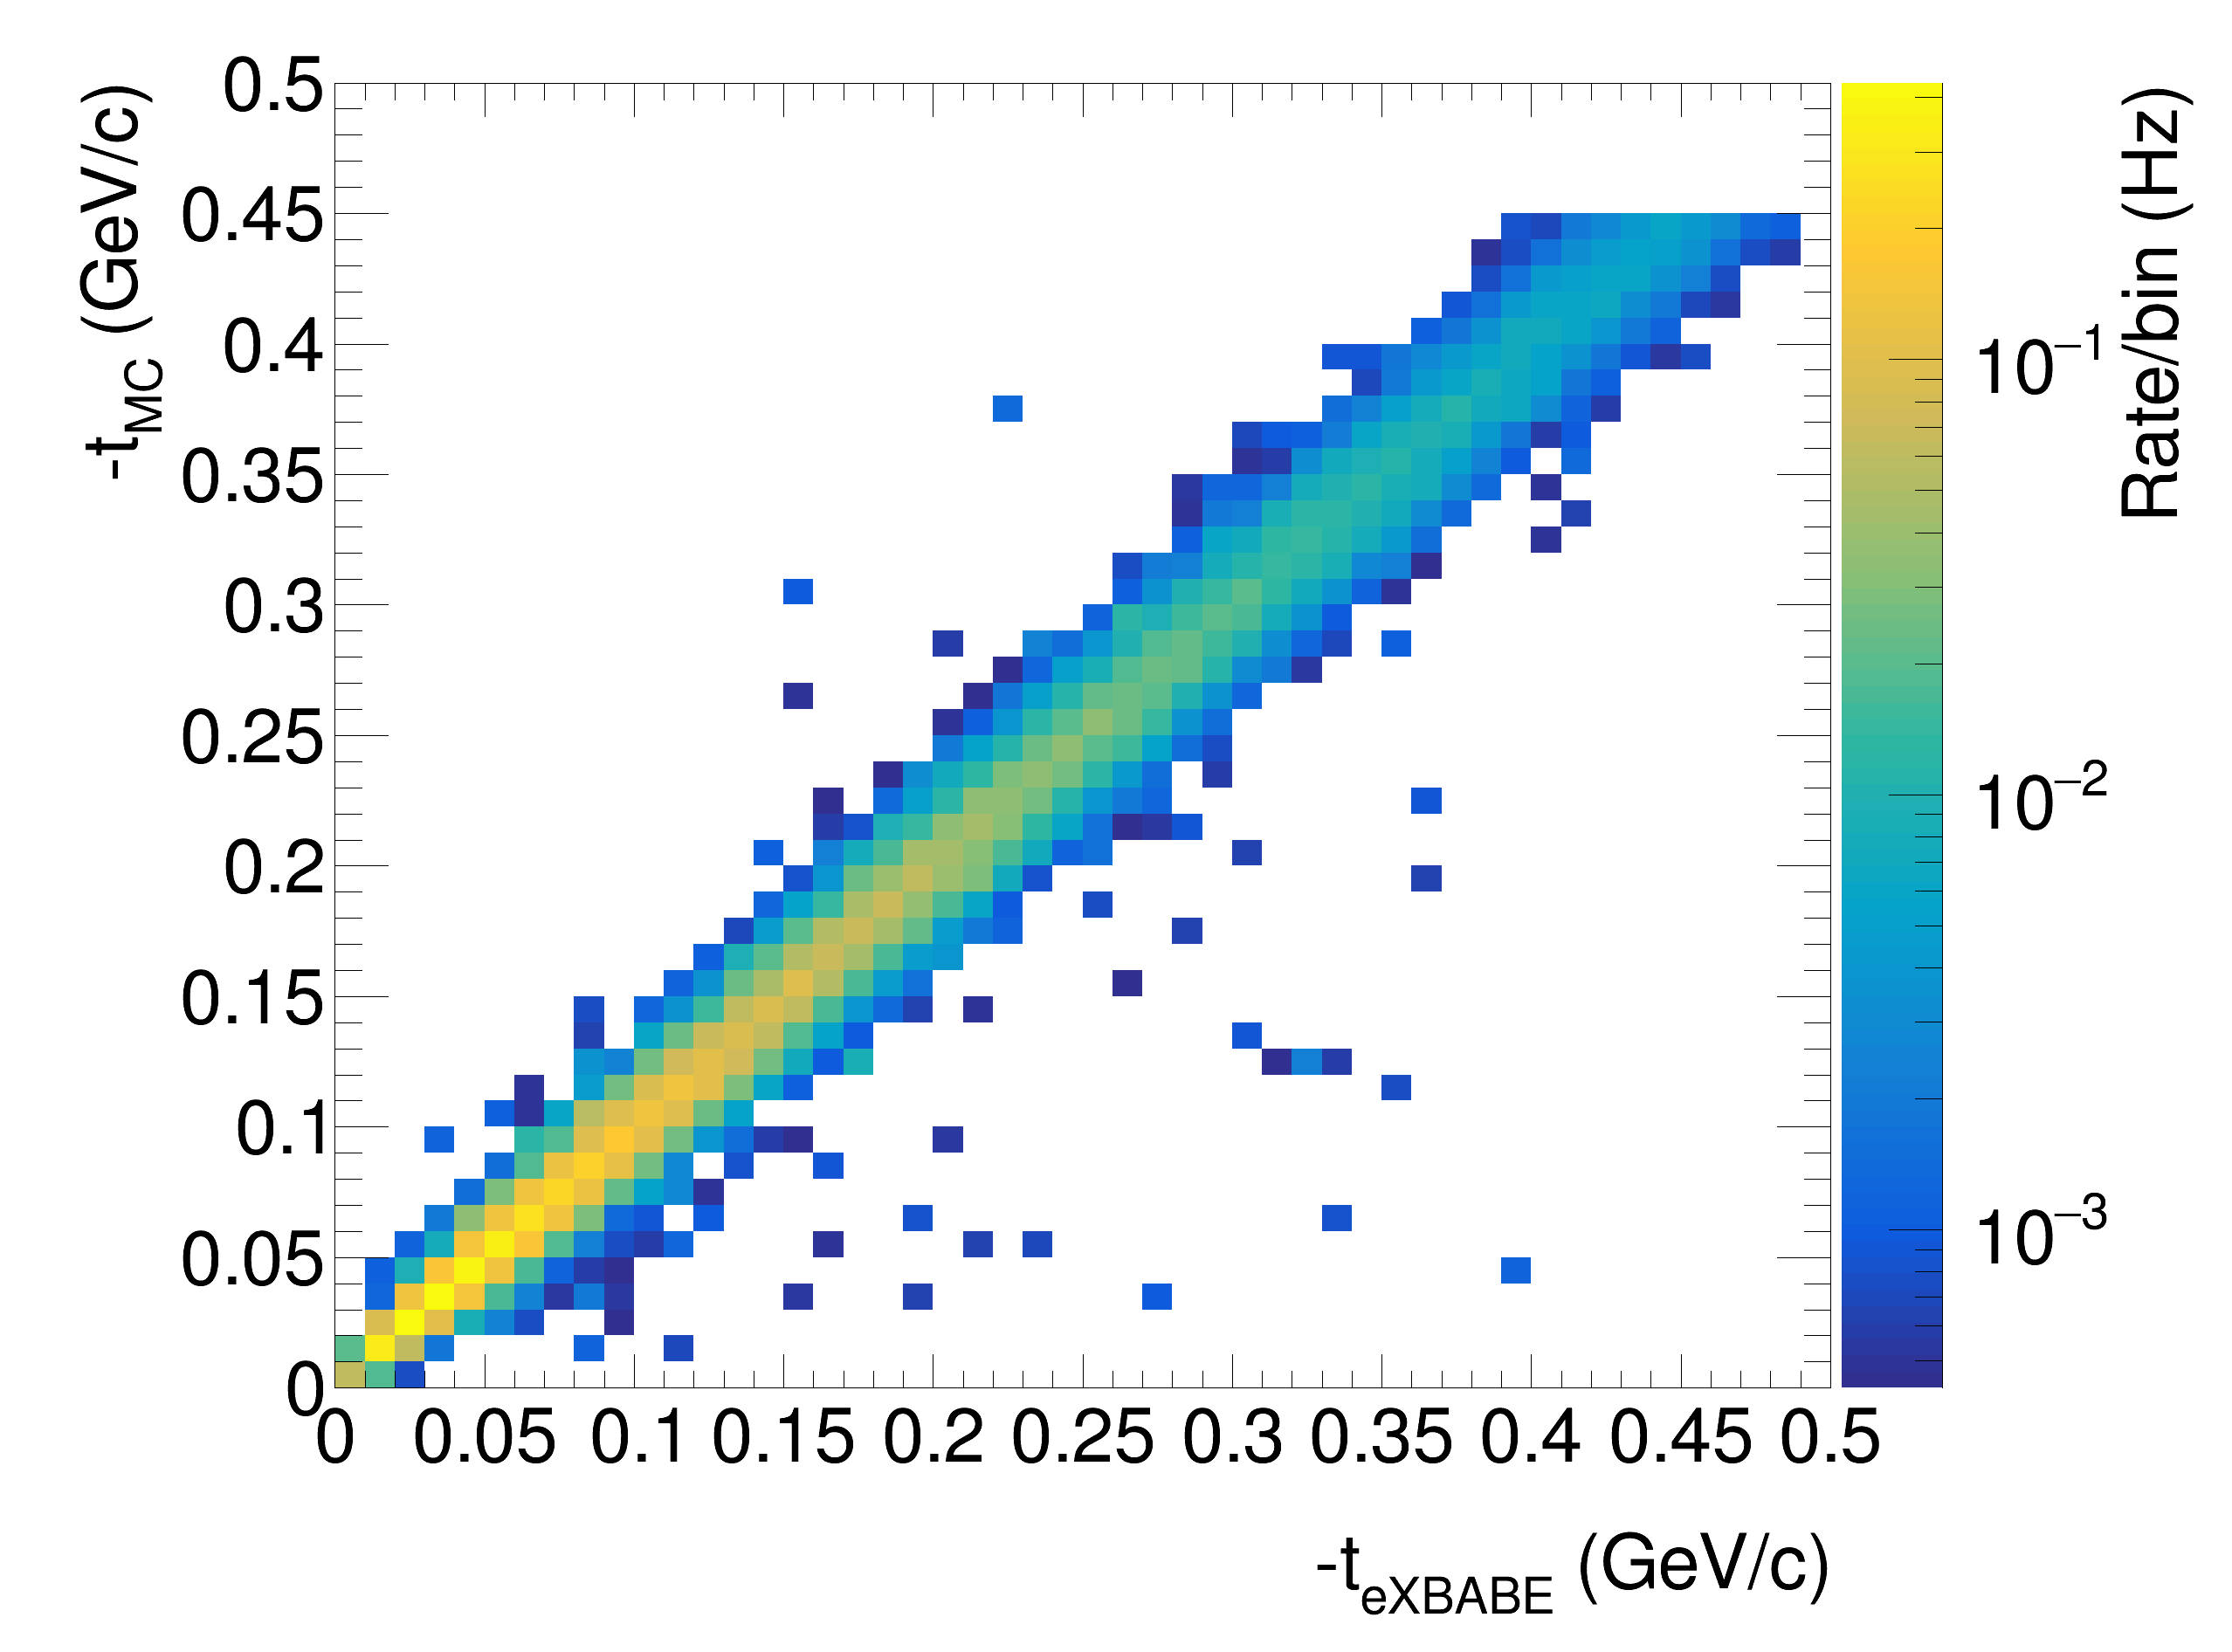
\includegraphics[width=0.475\textwidth]{Figures/10on250_tCompAlt_ZDC.png}
    \caption{A comparison of $-t_{eXBABE}$ against the MC truth value of $-t$ for 10x130 (left) and 10x250 (right) event samples. \textcolor{red}{Need to update units.}}
\label{fig:teXBABE_Comp}
\end{figure}

Once calculated, a cut is applied on $-t$. Any events with\newline $0~<~-t_{eXBABE}~<~1.4~(GeV/c)^{2}$ are removed. A cut on $W~>~0~GeV$ is also applied with any events failing this selection being removed. These cuts are applied simultaneously in conjunction with other cuts that are described in Sec.~\ref{subsec:Exclusivity_Cuts}.

\subsection{Event Selection - Final Cuts}\label{subsec:Exclusivity_Cuts}

To ensure exclusivity and remove background events, further cuts are needed. This DEMP analysis utilises a somewhat unique cut to achieve these objectives. To implement this cut, a missing momentum vector is determined from the reconstructed $e'$ and $\pi^{+}$ tracks -

\begin{gather*}
    \vec{P}_{Miss} = \left(\vec{e}+\vec{p}\right) - \left(\vec{e}\prime_{Rec} + \vec{\pi}_{Rec}\right)
\end{gather*}

where $\vec{e}$ and $\vec{p}$ are the initial electron and proton beam 4-vectors. If this is an exclusive event, the resulting four vector should correspond to the neutron. The polar and azimuthal ($\theta^{*}_{Miss}$ and $\phi^{*}_{Miss}$ angles of this track (after rotation by $25~mRad$ to remove beam crossing effects) should correspond to the polar and azimuthal angles determined from the neutron hit on the ZDC ($\theta^{*}_{ZDC}$ and $\phi^{*}_{ZDC}$, again, after rotation by $25~mRad$). Two differences, $\Delta\theta^{*}a$ and $\Delta\phi^{*}i$ can then be defined and calculated as -

\begin{gather*}
    \Delta\theta^{*} = \theta^{*}_{pMiss} - \theta^{*}_{ZDC},\\
    \Delta\phi^{*} = \phi^{*}_{PMiss} - \phi^{*}_{ZDC}.
\end{gather*}

For exclusive events, these differences should be very small, particularly $\Delta\theta^{*}$ due to the excellent position resolution of the ZDC. As such, only events satisfying -

\begin{gather*}
    -0.09^{\circ} < \Delta\theta^{*} < 0.14^{\circ},\\
    -55^{\circ}< \Delta\phi^{*} < 55^{\circ},
\end{gather*}

for 10x130 events and

\begin{gather*}
    -0.07^{\circ} < \Delta\theta^{*} < 0.17^{\circ},\\
    -80^{\circ}< \Delta\phi^{*} < 80^{\circ},
\end{gather*}

for 10x250 events are retained. These ranges were chosen to fit along lines of constant rate in a plot of $\Delta\theta^{*}$ vs $\Delta\phi^{*}$, such as in Fig.\ref{fig:10x130_DeltaCut}, to ensure no variations across the acceptance of the ZDC. They were also chosen so as to be conservative as SIDIS or other background events, which should not reconstruct in this range, will be excluded. For non-exclusive events, the missing momentum vector should not correspond to a single particle and as such, $\Delta\theta^{*}$ and $\Delta\phi^{*}$ should be spread across a much broader range.

\begin{figure}[h]
    \centering
    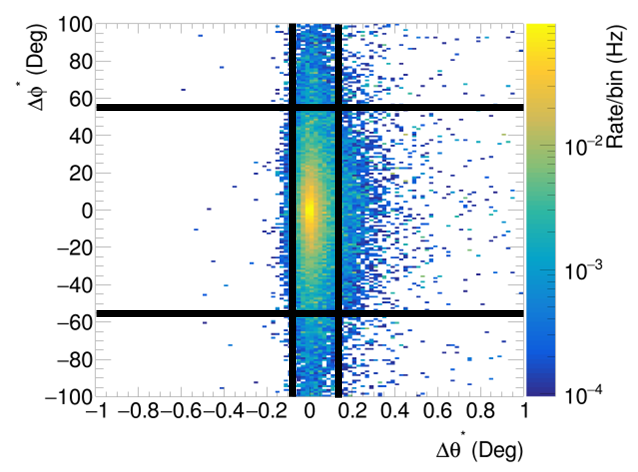
\includegraphics[width=\textwidth]{Figures/10x130_deltaTheta_deltaPhi_Cut.png}
    \caption{$\Delta\theta^{*}$ vs $\Delta\phi^{*}$ for 10x130 events. Note that as only DEMP events are processed, the majority of events survive this cut. Cuts were chosen along lines of constant rate as the peak area of the distribution tails off, as indicated by the solid black lines showing the cut region.}
\label{fig:10x130_DeltaCut}
\end{figure}

This cut is an indirect cut on the missing momentum and, as a consequence, the missing energy. As such, no additional cuts on the missing momentum or energy (which may be more typical of an exclusivity cut) are applied. The only other cut that is applied is a cut on the sum of $E-P_{z}$ for all detected final state particles. In the absence of initial state radiation or background events, this sum should be roughly equal to two times the electron beam energy ($20~GeV$ in each case under study here). As such, a cut of -

\begin{gather*}
    18 < \sum \left(E - P_{z}\right) < 22,
\end{gather*}

is applied. Again, as no initial state radiation is included in DEMPgen and no background events are included in the event sample, this range has been chosen to be conservative. This cut range will likely be tweaked and adjusted as these effects are incorporated in future studies.

\subsection{Analysis Code}\label{subsec:Analysis_Code}

The analysis of processed DEMP events is via a standard ROOT/C++ based macro. The analysis code is stored on GitHub and can be accessed \href{https://github.com/sjdkay/ePIC_DEMP_Analysis/blob/main/DEMP_Analysis.C}{here}\footnote{\url{https://github.com/sjdkay/ePIC_DEMP_Analysis/blob/main/DEMP_Analysis.C}}. This repository also contains some utility scripts that can be used to cut down the size of the reconstructed simulation output if desired. 

\section{Results and Discussion}\label{sec:Results_Discuss}

Your results with key performance plots etc. Consult checklist of key figures, see \href{https://docs.google.com/presentation/d/1bqz9_GPvPoW4oz1m8KvzuUhPJZBe_CfU5APMt0LjfaU/edit?slide=id.g3338e3f4b69_0_51#slide=id.g3338e3f4b69_0_51}{page three of this presentation} as an example of plots to include.

Once triple-coincidence $p(e,e'\pi^+n)$ events are cleanly identified with ePIC, the value of $F_{\pi}(Q^2)$ is determined by comparing the measured $d\sigma/dt$ values at small $-t$ to the best available electroproduction model. The obtained $F_{\pi}$ values are in principle dependent upon the model used, but one anticipates this dependence to be reduced at sufficiently small $-t$. Measurements over a range of $-t$ are an essential part of the model validation process. The JLab 6\,GeV experiments were instrumental in establishing the reliability of this technique up to $Q^2=2.45$~GeV$^2$~\cite{Huber:2008id, Horn:2016rip, Horn:2007ug, Volmer:2000ek, Horn:2006tm, Tadevosyan:2007yd, Blok:2008jy, Huber:2014ius, Huber:2014kar}, and extensive further tests are planned as part of JLab experiment E12-19-006 \cite{E12-19-006}.

{\bf GH can add more discussion later.}

\pagebreak
\appendix
\section{Appendix}
Material you wish to include in an appendix. 

\bibliographystyle{elsarticle-num} 
\bibliography{bibliography.bib}

\end{document}